\section{Simulation Analysis}\label{section:sim}
 In this section ngspice was used in order to simulate the ac/dc converter. Some modifications were made from the start in ordem to simplify the circuit.
 
 First of all, the transformer was replaced by an ideal model, and once the Vs value was used, using a depedent current source (instead of the primary) and a dependent voltage source, (insetad of the secundary). This allowed the group to not having to model a "real" transformer. 
 
Then, the values of n (parameter of dependency of the dependent sources), the capacitance of the capacitor and the values of the resistance of the resistors were being adjusted through trial and error in order to achieve a maximum accurary of the output voltage, since the initial goal was to get this value close as possible to 12 V.


In the table below, the Imput voltage of the secundary circuit (v(2)), output Voltage of the Envelope Detector (v(4)), the output voltage of the  Voltage Regulator (v(5)), and v(5)-12 were computed. This is a visual representation of the effect of the envelope detector, which decreases the ripple voltage and of the voltage regulator , that keeps the output voltage constant. As seen V(5)- 12 is a line (not completely straight due to the oscilations caused by the diodes, that are not linear components ) close to 0, that was the main goal of the assignment.

\begin{figure}[h] \centering
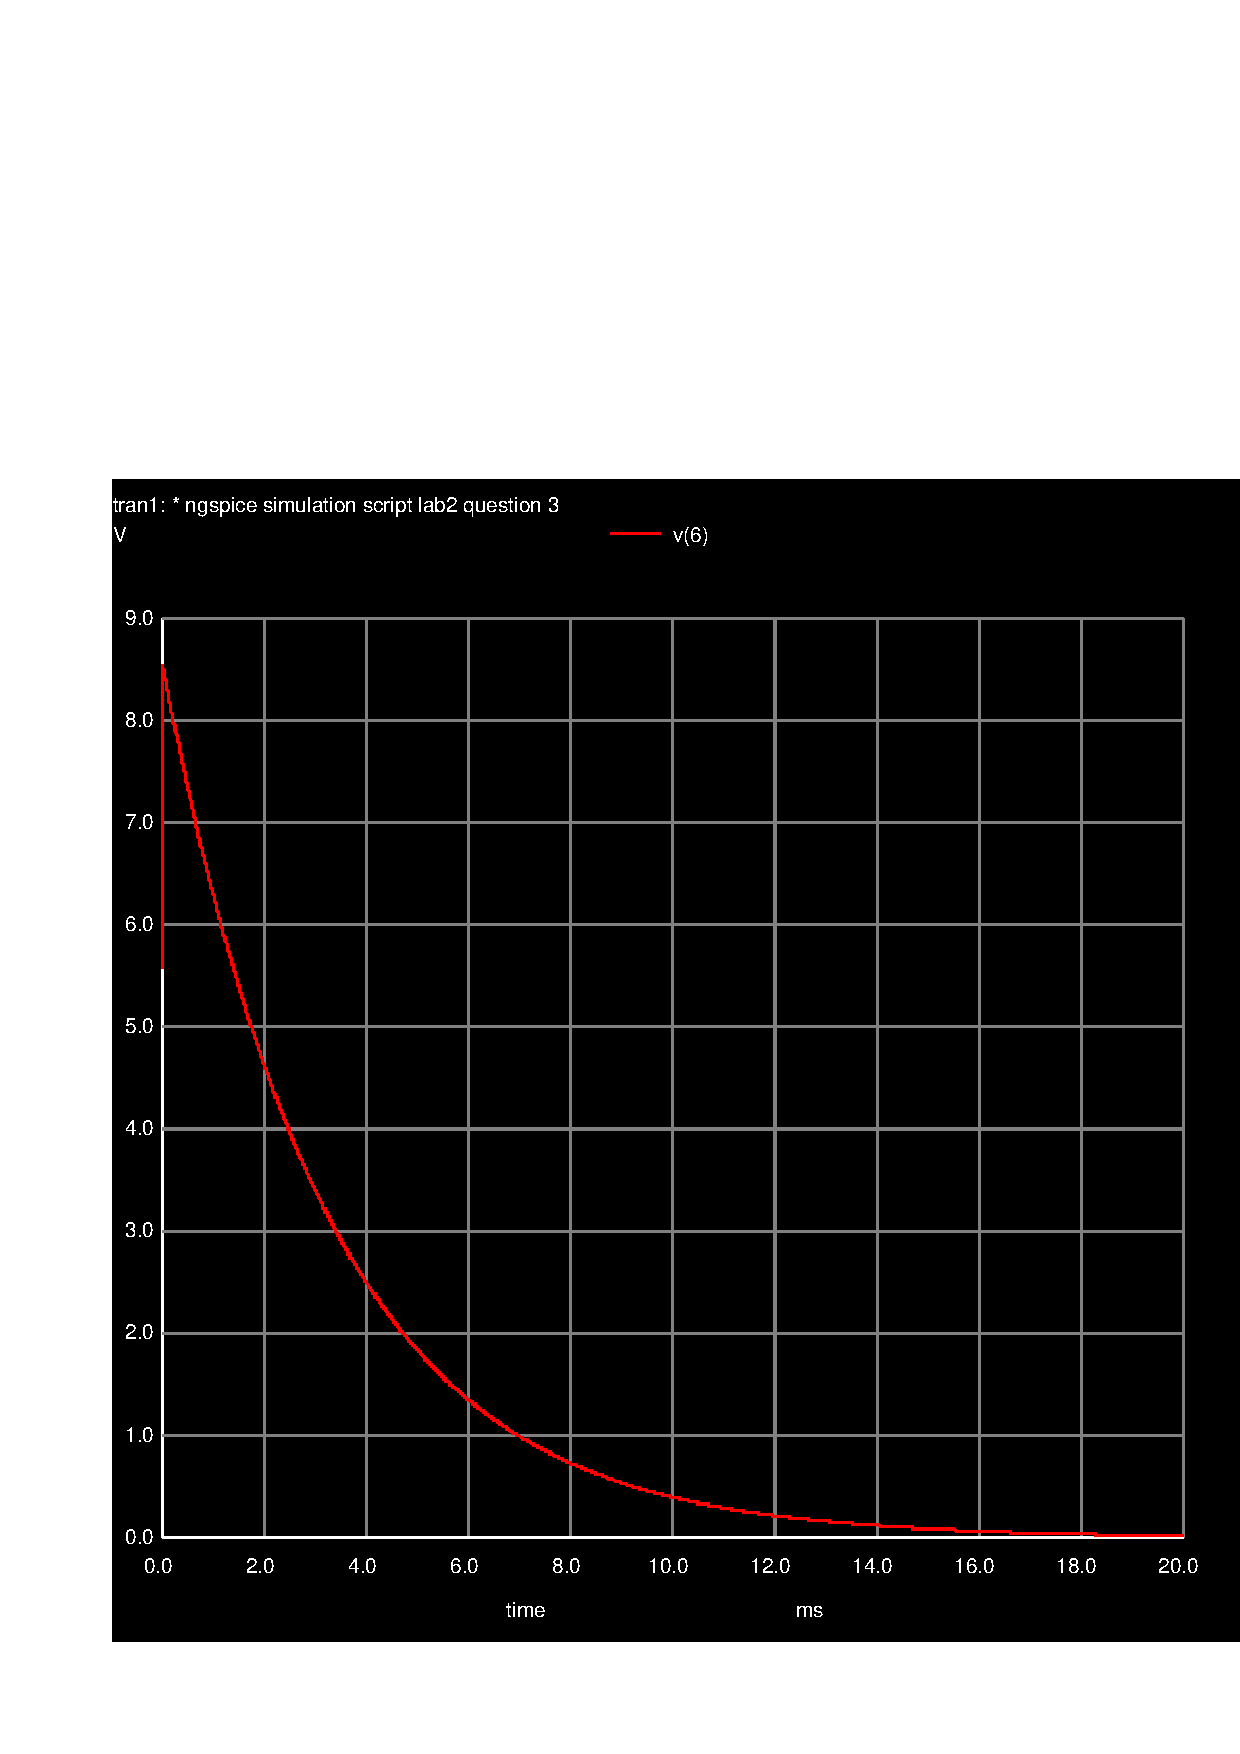
\includegraphics[width=0.3\linewidth]{sim3.pdf}
\caption{Imput voltage of the secundary circuit (v(2)), output Voltage of the Envelope Detector (v(4)), Voltage Regulator (v(5)), and v(5)-12}
\label{fig:sim5}
\end{figure}





